% Created by tikzDevice version 0.12 on 2019-06-14 22:23:46
% !TEX encoding = UTF-8 Unicode
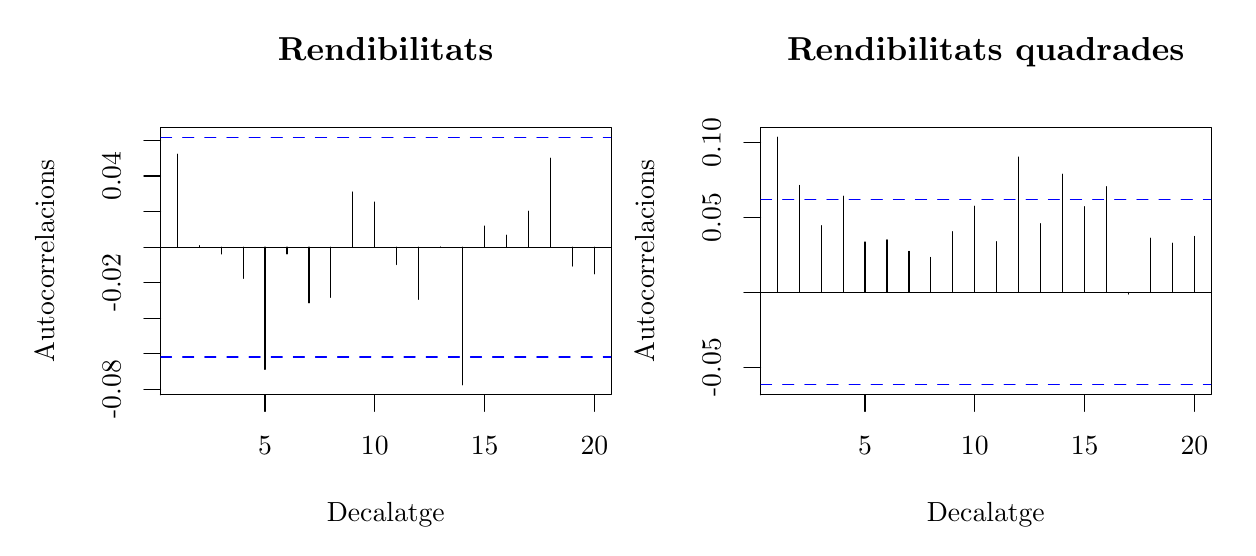
\begin{tikzpicture}[x=1pt,y=1pt]
\definecolor{fillColor}{RGB}{255,255,255}
\path[use as bounding box,fill=fillColor,fill opacity=0.00] (0,0) rectangle (433.62,180.67);
\begin{scope}
\path[clip] ( 48.00, 48.00) rectangle (210.81,144.67);
\definecolor{drawColor}{RGB}{0,0,0}

\path[draw=drawColor,line width= 0.4pt,line join=round,line cap=round] ( 54.03,101.38) -- ( 54.03,134.99);

\path[draw=drawColor,line width= 0.4pt,line join=round,line cap=round] ( 61.96,101.38) -- ( 61.96,101.90);

\path[draw=drawColor,line width= 0.4pt,line join=round,line cap=round] ( 69.90,101.38) -- ( 69.90, 98.90);

\path[draw=drawColor,line width= 0.4pt,line join=round,line cap=round] ( 77.83,101.38) -- ( 77.83, 90.11);

\path[draw=drawColor,line width= 0.4pt,line join=round,line cap=round] ( 85.77,101.38) -- ( 85.77, 57.20);

\path[draw=drawColor,line width= 0.4pt,line join=round,line cap=round] ( 93.70,101.38) -- ( 93.70, 98.91);

\path[draw=drawColor,line width= 0.4pt,line join=round,line cap=round] (101.64,101.38) -- (101.64, 81.23);

\path[draw=drawColor,line width= 0.4pt,line join=round,line cap=round] (109.57,101.38) -- (109.57, 83.22);

\path[draw=drawColor,line width= 0.4pt,line join=round,line cap=round] (117.50,101.38) -- (117.50,121.28);

\path[draw=drawColor,line width= 0.4pt,line join=round,line cap=round] (125.44,101.38) -- (125.44,117.66);

\path[draw=drawColor,line width= 0.4pt,line join=round,line cap=round] (133.37,101.38) -- (133.37, 95.10);

\path[draw=drawColor,line width= 0.4pt,line join=round,line cap=round] (141.31,101.38) -- (141.31, 82.54);

\path[draw=drawColor,line width= 0.4pt,line join=round,line cap=round] (149.24,101.38) -- (149.24,101.47);

\path[draw=drawColor,line width= 0.4pt,line join=round,line cap=round] (157.17,101.38) -- (157.17, 51.58);

\path[draw=drawColor,line width= 0.4pt,line join=round,line cap=round] (165.11,101.38) -- (165.11,108.99);

\path[draw=drawColor,line width= 0.4pt,line join=round,line cap=round] (173.04,101.38) -- (173.04,105.66);

\path[draw=drawColor,line width= 0.4pt,line join=round,line cap=round] (180.98,101.38) -- (180.98,114.38);

\path[draw=drawColor,line width= 0.4pt,line join=round,line cap=round] (188.91,101.38) -- (188.91,133.52);

\path[draw=drawColor,line width= 0.4pt,line join=round,line cap=round] (196.85,101.38) -- (196.85, 94.51);

\path[draw=drawColor,line width= 0.4pt,line join=round,line cap=round] (204.78,101.38) -- (204.78, 91.69);
\end{scope}
\begin{scope}
\path[clip] (  0.00,  0.00) rectangle (433.62,180.67);
\definecolor{drawColor}{RGB}{0,0,0}

\path[draw=drawColor,line width= 0.4pt,line join=round,line cap=round] ( 85.77, 48.00) -- (204.78, 48.00);

\path[draw=drawColor,line width= 0.4pt,line join=round,line cap=round] ( 85.77, 48.00) -- ( 85.77, 42.00);

\path[draw=drawColor,line width= 0.4pt,line join=round,line cap=round] (125.44, 48.00) -- (125.44, 42.00);

\path[draw=drawColor,line width= 0.4pt,line join=round,line cap=round] (165.11, 48.00) -- (165.11, 42.00);

\path[draw=drawColor,line width= 0.4pt,line join=round,line cap=round] (204.78, 48.00) -- (204.78, 42.00);

\node[text=drawColor,anchor=base,inner sep=0pt, outer sep=0pt, scale=  1.00] at ( 85.77, 26.40) {5};

\node[text=drawColor,anchor=base,inner sep=0pt, outer sep=0pt, scale=  1.00] at (125.44, 26.40) {10};

\node[text=drawColor,anchor=base,inner sep=0pt, outer sep=0pt, scale=  1.00] at (165.11, 26.40) {15};

\node[text=drawColor,anchor=base,inner sep=0pt, outer sep=0pt, scale=  1.00] at (204.78, 26.40) {20};

\path[draw=drawColor,line width= 0.4pt,line join=round,line cap=round] ( 48.00, 50.01) -- ( 48.00,139.90);

\path[draw=drawColor,line width= 0.4pt,line join=round,line cap=round] ( 48.00, 50.01) -- ( 42.00, 50.01);

\path[draw=drawColor,line width= 0.4pt,line join=round,line cap=round] ( 48.00, 62.85) -- ( 42.00, 62.85);

\path[draw=drawColor,line width= 0.4pt,line join=round,line cap=round] ( 48.00, 75.69) -- ( 42.00, 75.69);

\path[draw=drawColor,line width= 0.4pt,line join=round,line cap=round] ( 48.00, 88.53) -- ( 42.00, 88.53);

\path[draw=drawColor,line width= 0.4pt,line join=round,line cap=round] ( 48.00,101.38) -- ( 42.00,101.38);

\path[draw=drawColor,line width= 0.4pt,line join=round,line cap=round] ( 48.00,114.22) -- ( 42.00,114.22);

\path[draw=drawColor,line width= 0.4pt,line join=round,line cap=round] ( 48.00,127.06) -- ( 42.00,127.06);

\path[draw=drawColor,line width= 0.4pt,line join=round,line cap=round] ( 48.00,139.90) -- ( 42.00,139.90);

\node[text=drawColor,rotate= 90.00,anchor=base,inner sep=0pt, outer sep=0pt, scale=  1.00] at ( 33.60, 50.01) {-0.08};

\node[text=drawColor,rotate= 90.00,anchor=base,inner sep=0pt, outer sep=0pt, scale=  1.00] at ( 33.60, 88.53) {-0.02};

\node[text=drawColor,rotate= 90.00,anchor=base,inner sep=0pt, outer sep=0pt, scale=  1.00] at ( 33.60,127.06) {0.04};

\path[draw=drawColor,line width= 0.4pt,line join=round,line cap=round] ( 48.00, 48.00) --
	(210.81, 48.00) --
	(210.81,144.67) --
	( 48.00,144.67) --
	( 48.00, 48.00);
\end{scope}
\begin{scope}
\path[clip] (  0.00,  0.00) rectangle (216.81,180.67);
\definecolor{drawColor}{RGB}{0,0,0}

\node[text=drawColor,anchor=base,inner sep=0pt, outer sep=0pt, scale=  1.00] at (129.40,  2.40) {Decalatge};

\node[text=drawColor,rotate= 90.00,anchor=base,inner sep=0pt, outer sep=0pt, scale=  1.00] at (  9.60, 96.34) {Autocorrelacions};
\end{scope}
\begin{scope}
\path[clip] ( 48.00, 48.00) rectangle (210.81,144.67);
\definecolor{drawColor}{RGB}{0,0,0}

\path[draw=drawColor,line width= 0.4pt,line join=round,line cap=round] ( 48.00,101.38) -- (210.81,101.38);
\definecolor{drawColor}{RGB}{0,0,255}

\path[draw=drawColor,line width= 0.4pt,dash pattern=on 4pt off 4pt ,line join=round,line cap=round] ( 48.00,141.09) -- (210.81,141.09);

\path[draw=drawColor,line width= 0.4pt,dash pattern=on 4pt off 4pt ,line join=round,line cap=round] ( 48.00, 61.66) -- (210.81, 61.66);
\end{scope}
\begin{scope}
\path[clip] (  0.00,  0.00) rectangle (216.81,180.67);
\definecolor{drawColor}{RGB}{0,0,0}

\node[text=drawColor,anchor=base,inner sep=0pt, outer sep=0pt, scale=  1.20] at (129.40,168.67) {\bfseries Rendibilitats};
\end{scope}
\begin{scope}
\path[clip] (264.81, 48.00) rectangle (427.62,144.67);
\definecolor{drawColor}{RGB}{0,0,0}

\path[draw=drawColor,line width= 0.4pt,line join=round,line cap=round] (270.84, 85.03) -- (270.84,141.09);

\path[draw=drawColor,line width= 0.4pt,line join=round,line cap=round] (278.77, 85.03) -- (278.77,123.67);

\path[draw=drawColor,line width= 0.4pt,line join=round,line cap=round] (286.71, 85.03) -- (286.71,109.10);

\path[draw=drawColor,line width= 0.4pt,line join=round,line cap=round] (294.64, 85.03) -- (294.64,119.79);

\path[draw=drawColor,line width= 0.4pt,line join=round,line cap=round] (302.58, 85.03) -- (302.58,103.23);

\path[draw=drawColor,line width= 0.4pt,line join=round,line cap=round] (310.51, 85.03) -- (310.51,103.99);

\path[draw=drawColor,line width= 0.4pt,line join=round,line cap=round] (318.45, 85.03) -- (318.45, 99.84);

\path[draw=drawColor,line width= 0.4pt,line join=round,line cap=round] (326.38, 85.03) -- (326.38, 97.63);

\path[draw=drawColor,line width= 0.4pt,line join=round,line cap=round] (334.31, 85.03) -- (334.31,106.94);

\path[draw=drawColor,line width= 0.4pt,line join=round,line cap=round] (342.25, 85.03) -- (342.25,116.20);

\path[draw=drawColor,line width= 0.4pt,line join=round,line cap=round] (350.18, 85.03) -- (350.18,103.36);

\path[draw=drawColor,line width= 0.4pt,line join=round,line cap=round] (358.12, 85.03) -- (358.12,133.92);

\path[draw=drawColor,line width= 0.4pt,line join=round,line cap=round] (366.05, 85.03) -- (366.05,109.86);

\path[draw=drawColor,line width= 0.4pt,line join=round,line cap=round] (373.98, 85.03) -- (373.98,127.74);

\path[draw=drawColor,line width= 0.4pt,line join=round,line cap=round] (381.92, 85.03) -- (381.92,115.98);

\path[draw=drawColor,line width= 0.4pt,line join=round,line cap=round] (389.85, 85.03) -- (389.85,123.24);

\path[draw=drawColor,line width= 0.4pt,line join=round,line cap=round] (397.79, 85.03) -- (397.79, 84.38);

\path[draw=drawColor,line width= 0.4pt,line join=round,line cap=round] (405.72, 85.03) -- (405.72,104.57);

\path[draw=drawColor,line width= 0.4pt,line join=round,line cap=round] (413.66, 85.03) -- (413.66,102.79);

\path[draw=drawColor,line width= 0.4pt,line join=round,line cap=round] (421.59, 85.03) -- (421.59,105.26);
\end{scope}
\begin{scope}
\path[clip] (  0.00,  0.00) rectangle (433.62,180.67);
\definecolor{drawColor}{RGB}{0,0,0}

\path[draw=drawColor,line width= 0.4pt,line join=round,line cap=round] (302.58, 48.00) -- (421.59, 48.00);

\path[draw=drawColor,line width= 0.4pt,line join=round,line cap=round] (302.58, 48.00) -- (302.58, 42.00);

\path[draw=drawColor,line width= 0.4pt,line join=round,line cap=round] (342.25, 48.00) -- (342.25, 42.00);

\path[draw=drawColor,line width= 0.4pt,line join=round,line cap=round] (381.92, 48.00) -- (381.92, 42.00);

\path[draw=drawColor,line width= 0.4pt,line join=round,line cap=round] (421.59, 48.00) -- (421.59, 42.00);

\node[text=drawColor,anchor=base,inner sep=0pt, outer sep=0pt, scale=  1.00] at (302.58, 26.40) {5};

\node[text=drawColor,anchor=base,inner sep=0pt, outer sep=0pt, scale=  1.00] at (342.25, 26.40) {10};

\node[text=drawColor,anchor=base,inner sep=0pt, outer sep=0pt, scale=  1.00] at (381.92, 26.40) {15};

\node[text=drawColor,anchor=base,inner sep=0pt, outer sep=0pt, scale=  1.00] at (421.59, 26.40) {20};

\path[draw=drawColor,line width= 0.4pt,line join=round,line cap=round] (264.81, 57.99) -- (264.81,139.11);

\path[draw=drawColor,line width= 0.4pt,line join=round,line cap=round] (264.81, 57.99) -- (258.81, 57.99);

\path[draw=drawColor,line width= 0.4pt,line join=round,line cap=round] (264.81, 85.03) -- (258.81, 85.03);

\path[draw=drawColor,line width= 0.4pt,line join=round,line cap=round] (264.81,112.07) -- (258.81,112.07);

\path[draw=drawColor,line width= 0.4pt,line join=round,line cap=round] (264.81,139.11) -- (258.81,139.11);

\node[text=drawColor,rotate= 90.00,anchor=base,inner sep=0pt, outer sep=0pt, scale=  1.00] at (250.41, 57.99) {-0.05};

\node[text=drawColor,rotate= 90.00,anchor=base,inner sep=0pt, outer sep=0pt, scale=  1.00] at (250.41,112.07) {0.05};

\node[text=drawColor,rotate= 90.00,anchor=base,inner sep=0pt, outer sep=0pt, scale=  1.00] at (250.41,139.11) {0.10};

\path[draw=drawColor,line width= 0.4pt,line join=round,line cap=round] (264.81, 48.00) --
	(427.62, 48.00) --
	(427.62,144.67) --
	(264.81,144.67) --
	(264.81, 48.00);
\end{scope}
\begin{scope}
\path[clip] (216.81,  0.00) rectangle (433.62,180.67);
\definecolor{drawColor}{RGB}{0,0,0}

\node[text=drawColor,anchor=base,inner sep=0pt, outer sep=0pt, scale=  1.00] at (346.21,  2.40) {Decalatge};

\node[text=drawColor,rotate= 90.00,anchor=base,inner sep=0pt, outer sep=0pt, scale=  1.00] at (226.41, 96.34) {Autocorrelacions};
\end{scope}
\begin{scope}
\path[clip] (264.81, 48.00) rectangle (427.62,144.67);
\definecolor{drawColor}{RGB}{0,0,0}

\path[draw=drawColor,line width= 0.4pt,line join=round,line cap=round] (264.81, 85.03) -- (427.62, 85.03);
\definecolor{drawColor}{RGB}{0,0,255}

\path[draw=drawColor,line width= 0.4pt,dash pattern=on 4pt off 4pt ,line join=round,line cap=round] (264.81,118.48) -- (427.62,118.48);

\path[draw=drawColor,line width= 0.4pt,dash pattern=on 4pt off 4pt ,line join=round,line cap=round] (264.81, 51.58) -- (427.62, 51.58);
\end{scope}
\begin{scope}
\path[clip] (216.81,  0.00) rectangle (433.62,180.67);
\definecolor{drawColor}{RGB}{0,0,0}

\node[text=drawColor,anchor=base,inner sep=0pt, outer sep=0pt, scale=  1.20] at (346.21,168.67) {\bfseries Rendibilitats quadrades};
\end{scope}
\end{tikzpicture}
